\renewcommand{\thefootnote}{\fnsymbol{footnote}}


\section{Features}

% (Should we present this information in a bullet list or in paragraphs?)
%
% \begin{enumerate}
%
% \item Map View - easy navigation and quick browsing
%
%   \begin{itemize}
%
%   \item Pan and zoom the sky map by dragging and scrolling
%
%   \item Toggle and view specific catalog layers and multi-wavelength survey images
%
%   \item Pop-ups over each source for basic information
%
%   \item Powerful search tools - locate objects by name, association, or coordinate position
%
%   \item Export and share a specific view of the sky map via PNG
%
%   \end{itemize}
%
%
% \item Catalog View - deeply investigate a specific source
%
%   \begin{itemize}
%
%   \item Search tool to find a source in its respective catalog by source name
%
%   \item Basic info, extension info, spectral info, distance info
%
%   \item Light curves, emission spectra (currently only for 3FGL catalog)
%
%   \item References to which telescope detected the source and links to where our data came from
%
%   \end{itemize}
%
%
% \item Further analysis of our data with tools like Gammapy (generate specific plots, etc.)
%
% \item Mention again that all data is openly available for download
%
% \end{enumerate}


  The items listed below illustrate the interface of gamma-sky.net and its utilization as a tool for astronomers.

  \begin{enumerate}

    \item \textbf{Browsing and navigation features} in the Map View component:

      \begin{itemize}

        \item Pan and zoom
        \item Search tools - locate objects by name, association, or coordinate position
        \item Toggle and view specific catalog layers and sky images
        \item Pop-up information over each source
        \item Export and share images from the sky map (in PNG format)

      \end{itemize}

    \item \textbf{Analysis tools} in the Catalog View component\footnote[1]{Some of the features listed for the Catalog View are currently only available for select catalogs, but they are expected to be a part of all catalogs in the near future.}:

      \begin{itemize}

        \item Search and select a source by its name
        \item Basic information - position, association and class
        \item Extension information
        \item Spectral index, brightness and flux
        \item Distance and redshift
        \item Graphs of light curves and emission spectra
        \item Detection/observation information - instrument, date of discovery and relevant papers

      \end{itemize}

  \end{enumerate}


  TODO: How does this features list look? Should we make it more ``elegant"/space them out a bit?


  TODO: Fix image placement after all other text is finalized.


  \begin{figure}[t]
    \centerline{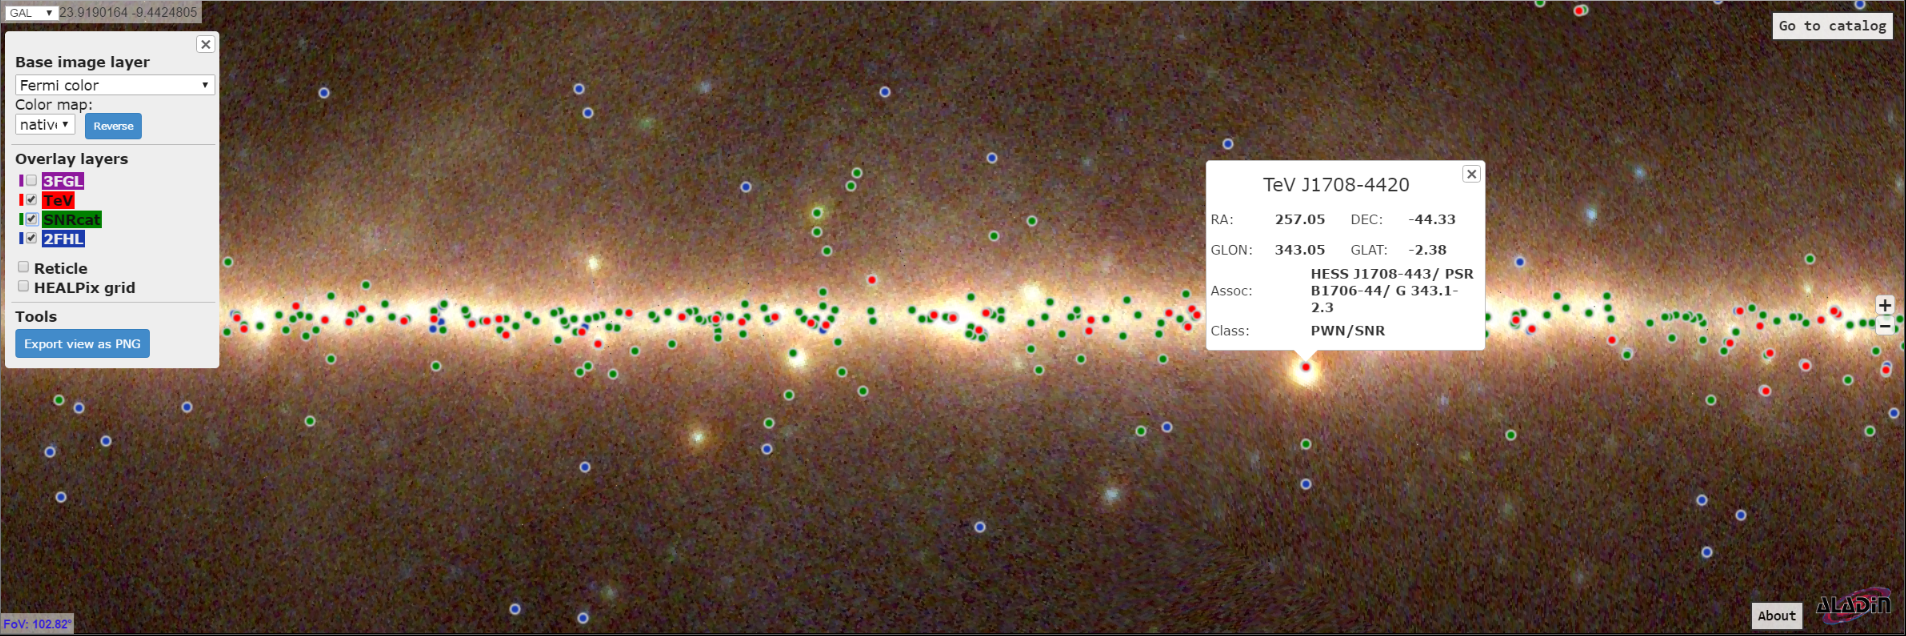
\includegraphics[width=\textwidth]{figures/mapview_wide}}
    \caption{Map View.}
    \label{fig:mapview}
  \end{figure}

  \begin{figure}[t]
    \centerline{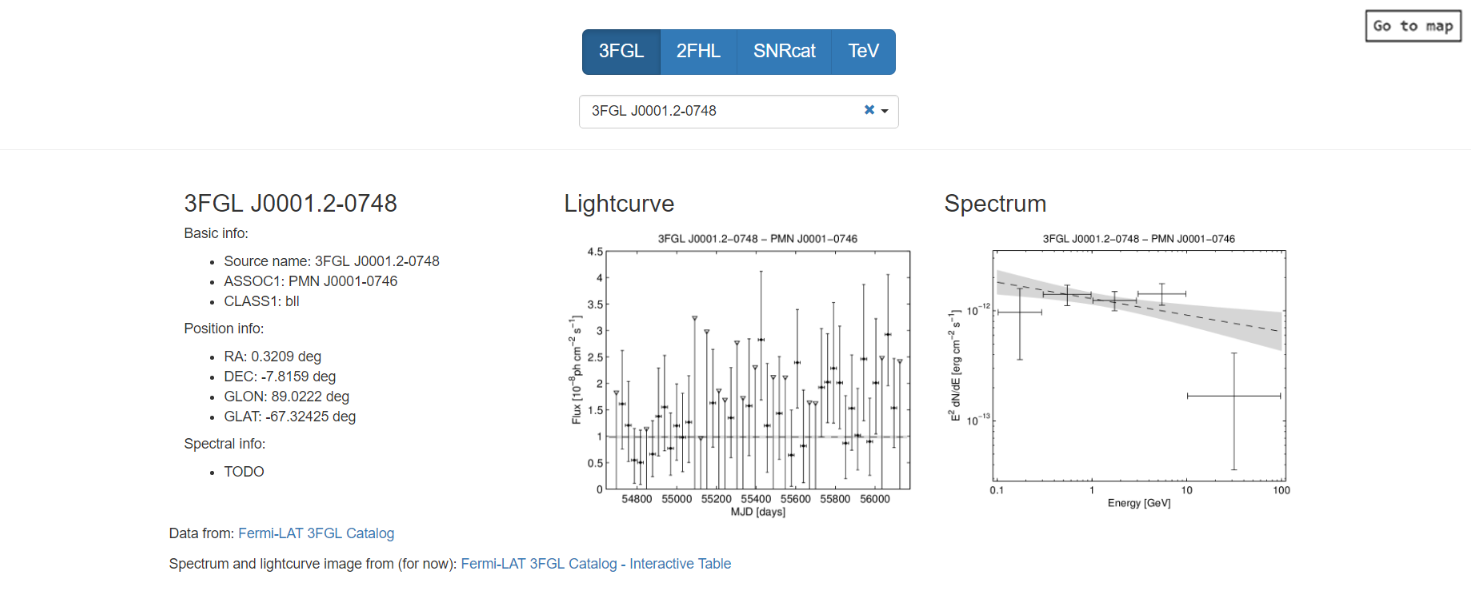
\includegraphics[width=\textwidth]{figures/catview_wide_zoom}}
    \caption{Catalog View.}
    \label{fig:catview}
  \end{figure}
